\documentclass[11pt]{article}

% useful packages
\usepackage{fullpage} % sets more standardized margins
\usepackage{graphicx} % some graphics functions 
\usepackage{tocloft}  % single space table of contents
\usepackage[title,toc,page]{appendix}
\usepackage[nottoc]{tocbibind}
\usepackage{fancyhdr}
\usepackage{wrapfig}
\usepackage{multirow}
\usepackage{lastpage}
\usepackage{hyperref}
\usepackage{xcolor}
\hypersetup{
    colorlinks,
    linkcolor={red!55!black},
    citecolor={blue!50!black},
    urlcolor={blue!80!black}
}

\usepackage{fontspec}
\setmainfont{Arial}

% to comport to IEEE style for referenceing figures
\usepackage{caption}
\usepackage[figurename=Fig.]{caption}
\captionsetup{labelsep = period}
\captionsetup[table]{labelsep=newline}
\captionsetup[table]{name=TABLE}
\renewcommand{\thetable}{\Roman{table}}
\captionsetup[figure]{labelsep=period}

% paragraph indentation and separation
\parindent = 0.0in  
\parskip = 12pt
%\renewcommand{\absnamepos}{flushleft} % left justifies abstract

% use Arial font
%\usepackage{fontspec}
%\setmainfont{Arial}

% header and footer
\renewcommand{\headrulewidth}{0.0pt}
\renewcommand{\footrulewidth}{0.4pt}
\lfoot{{\fontsize{10}{11} \selectfont ECE 214 - DC--DC Power Supply}}
\cfoot{}
\rfoot{\fontsize{10}{11} \selectfont \thepage\ of \pageref{LastPage}}
\lhead{}
\chead{}
\rhead{}
\pagestyle{fancy}

\begin{document}

% Title and autheor
\title{ \textbf{ECE 214 Lab Report}\\
	Lab Title}
\author{Author 1\\
  	Author 2}
\date{\today}
\maketitle
\thispagestyle{empty}
\pagenumbering{roman}

% Abstract 
\section*{Abstract}
\noindent In the abstract, give the reader a general idea of what the lab and report are about. The abstract should be on your cover page. Highlight the major sections of the circuit without going into too much detail. The abstract should stand alone, meaning that the reader should not have to look at the report itself to get an idea of what the report is about. Additionally, provide one or two of the most important results you obtained in lab. For example, if you built a DC--DC power supply, you would indicate that the power supply had a DC input of 10~V, and produced a DC output of 25~V with an ac ripple of xx~mV at a fundamental frequency of yy~kHz. Some ways to begin the abstract include:
``The design, construction, and testing of a [circuit] is described.''
``A [circuit] was designed, built, and tested.''
On another note, when you list the names of the authors, list them in alphabetical order by last name.


\newpage
\tableofcontents

\newpage
\listoffigures

\newpage
\listoftables

\newpage 
\pagenumbering{arabic} % Turn on page numbering

% Introduction section
\section{Introduction}
This is a draft template for the ECE 214 Report. It was adapted from a template created a few ago by Casey Clark for the ECE 342 lab reports. It is a work in progress; I hope it helps.

The introduction is kind of what it sounds like – an introduction to the report. State the purpose or main goal of the lab. Provide some discussion on things like the parts of the circuit (e.g. your DC-DC circuit is made of the boost circuit, astable multivibrator, etc.). It is a good idea to give some background theory (if there is any) just to make sure your reader is familiarized with your lab a little more.

In this section, you should list any requirements or specifications pertaining to the lab. For example, if you are designing an amplifier you needed to have a certain gain at a specific frequency, you would list the specification here. You can also preview your results here. 

At the end of the introduction, forecast the remainder of the sections. This does not have to be an exhaustive list, just a brief overview of the major report sections so the reader knows what to expect. Here is an example:
Section~\ref{design_section} of this report describes the theory of the circuits in the DC--DC power supply. Simulation results are shown in Section~\ref{sim_section}, and the experimental results in Section~\ref{exp_section}. A discussion of the results, sources of error, and possible improvements are provided in Section~\ref{dis_section}. A cost analysis is provided in Section~\ref{cost_section}, and conclusions are presented in Section~\ref{con_section}.

% Design and analysis section
\section{Circuit Design and Analysis}
\label{design_section}

After each big section header, make sure you include a few sentences of mini-introductory material about the section. Do not put the little section header right after the big section header. Include a block diagram or a detailed schematic if it helps explain how the parts of the circuit fit together.

% here is an example of including a figure with a caption in the report
\begin{figure}[ht]
\centering
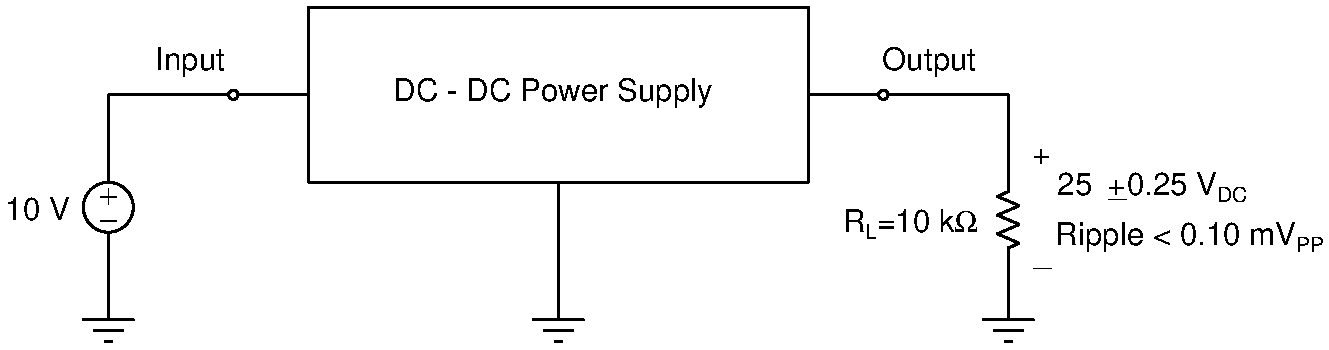
\includegraphics[width=5in]{dcdc_block}
\caption{Block diagram of the DC--DC power supply. Note: figure captions should be complete sentences and end in a period; they should not be sentence fragments.}
\label{block}
\end{figure}

Figures, equations, and tables should be numbered sequentially. Make sure all figures, equations, and tables are referenced and described in detail in the text. See the {\tt .tex} file for how to reference a figure. 

The text should say something like: Fig.~\ref{block} shows a block diagram of the DC--DC power supply. The input to the supply is a 10~V DC source. The power supply produces a DC output voltage of $25 \pm 0.25$~V when driving a 10~k$\Omega$ resistive load. The AC ripple is less than 0.10~mV$_{pp}$ with a fundamental frequency of xx~kHz. When including numbers in the report, always put the units right next to the numbers themselves.



\subsection{Boost Converter Circuit and Analysis}

Discuss how you designed your circuit in this section. Describe how you determined component values, frequencies, time-constants, etc. This section, as well as the majority of the report, should be in past tense because you are describing what you did. Furthermore, never use first or second person in your report. Always use third person. You might want to start out with a schematic of the circuit (or a portion of the circuit) to give your reader a visual. 

% another figure with a reference using the ECE214_Report_Template.bib file
\begin{figure}[ht]
\centering
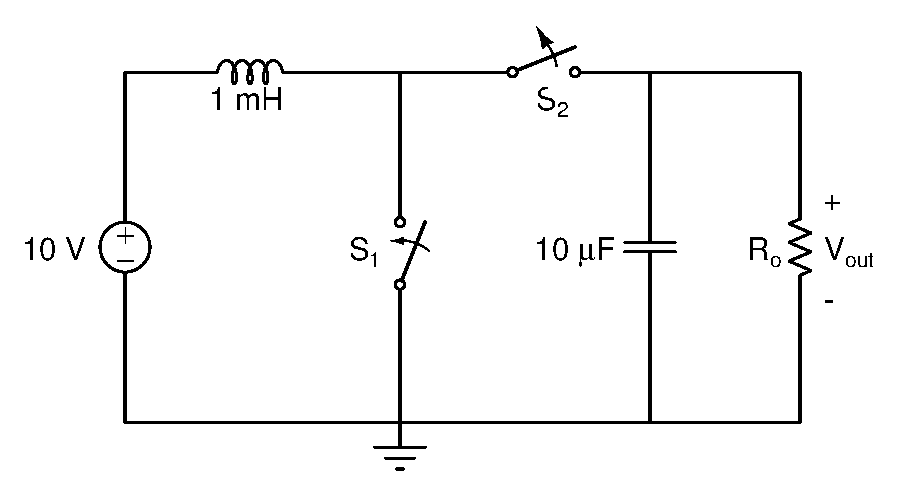
\includegraphics[width=4in]{boostcircuit}
\caption{Basic boost circuit using an ideal switch (taken from ECE214 Lab 7 instructions~\cite{ECE214_lab7}).}
\label{boostconverter}
\end{figure}

Do not put figures in the middle of a sentence. It is usually best to finish a sentence before putting in a figure. When you refer to figures in the text, you can say something like: ``The boost circuit shown in Fig.~\ref{boostconverter} was used to increase the DC voltage from 10~V to 25~V.'' Alternatively, you could say something like, ``To increase the DC voltage from 10~V to 25~V, the boost converter circuit was used (Fig.~\ref{boostconverter}).'' Make sure you capitalize ``Fig.'' Include a detailed description of all figures in the text.  

To create professional looking schematics, use software tools like Eagle, Altium, iCircuit, or Xcircuit. 

\textbf{References} should be used as necessary throughout the text. If you use information from any source that you did not create, it should be referenced. References are handled automatically by \LaTeX\ using the {\tt BitTex} tool. All bibliographic information is contained in a separate {\tt(.bib)} file. The file {\tt ECE214\_Report.bib} contains examples bibliographic entries for journal articles, conference proceedings, theses, and miscellaneous items. References are cited using their label. For example, to cite the reference with the label {\tt gunturi:2016b}, use the text: 
\vspace{-3mm}
\begin{verbatim}
In~\cite{gunturi:2016b}, the results of a UWB transmitter were described
\end{verbatim}
to produce:  ``In~\cite{gunturi:2016b}, the results of a UWB transmitter were described'' and reference~[2] is automatically added to the reference section on page \pageref{LastPage} of the report.  

Typical sub-sections for the Boost Converter section will include: 
\subsubsection{Calculation of Time for Current to Flow Into the Inductor}

\subsubsection{Calculation of Time for Current to Flow Out of the Inductor}

\subsubsection{Calculation and Selection of Output Resistor}

Further sub-sections for the Circuit Design and Analysis section of the report will include:

\subsection{Astable Multivibrator Circuit and Analysis}

\subsubsection{Calculation of Frequency and Duty Cycle}

\subsubsection{Selection of Capacitors Values}

\subsection{Low Pass Filter Circuit and Analysis}

\subsection{Complete DC--DC Power Supply Circuit and Analysis}


\textbf{Equations} should be placed on a separate line and numbered sequentially. Equations can be entered using the equation function in \LaTeX\ which will automatically number the equations. For example, to produce the equation below:  
\begin{equation}
A_{d} = \frac{v_{o1} - v_{o2}}{v_{id}} = -g_{m}(r_{oN}||r_{oP}).
\label{master_equation}
\end{equation}
the following \LaTeX\ code is entered: 
\begin{verbatim}
\begin{equation}
A_{d} = \frac{v_{o1} - v_{o2}}{v_{id}} = -g_{m}(r_{oN}||r_{oP}).
\label{master_equation}
\end{equation}
\end{verbatim}


When you refer to equations in the text, you can either use just the equation number (\ref{master_equation}) or say ``Eq.~(\ref{master_equation})'' or ``eq.~(\ref{master_equation}).'' However, be consistent and use the same convention throughout the report. 

Providing the equation with a label makes it easy to reference. In the example above, the equation was given the label: \begin{verbatim}\label{master_equation}\end{verbatim} that was then referenced as:
\begin{verbatim}
Eq.~(\ref{master_equation})
\end{verbatim}
to produce: Eq.~(\ref{master_equation}).

As with figures, try to avoid putting an equation in the middle of a sentence. It can be awkward and you run the risk of writing an incomplete sentence. Instead, try inserting the equation at the end of the sentence. For example:

The inverting integrating amplifier produces an output given by:
\begin{equation}
v_{out}(t) = - \frac{1}{RC} \int_0^\infty v_{in}(t) dt \, + v_{out}(0).
\label{deamp}
\end{equation}

Always define the variables in an equation, unless previously defined. Typically you mention the equation, show the equation, then define the variables in the equation.  For example, after Eq.~(\ref{deamp}) you would say something like; ``where $R$ is the resistance at the input to the amplifier; $C$ is the capacitance in the feedback loop of the amplifier, $t$ is time, and $V_{out}(0)$ is the initial output voltage.''


% Simulations
\section{Simulated Performance}
\label{sim_section}

Place your simulation results here. Again, do not forget to add a little blurb here about this section. You can say things like you did simulations in NGspice, the resistor values needed to be adjusted in simulations, and so on. Just avoid having section titles one right after the other. Do not forget to use past tense and third person too. 

Generally speaking, if you split up your circuit in a certain way in Section~\ref{design_section}, you should report the simulation results in a similar way. For the DC--DC converter, you might have Section 2.1 describing the boost converter, Section 2.2 describing the astable multivibrator, and Section 2.3 describing the low pass filter. Then, in this section, you would have a Section 3.1 describing the simulation results for the boost converter, Section 3.2 describing the simulation results for the astable multivibrator, and Section 3.3 describing the simulation results for the low pass filter. This is not always the case, but it is a good starting point if you are stuck on how to format things. Typical sub-sections might be:

\subsection{Boost Converter Simulation}

\subsection{Astable Multivibrator Simulation}

\subsection{Low Pass Filter Simulation}

\subsection{DC-DC Power Supply Simulation}

Also, when you are reporting simulation data, make sure the figures and graphs are clear. For example, if you have two lines on one graph, say that the blue line is voltage and the red line is current (or whatever). That way the reader knows what he/she is looking at. Also, label your axes. It sounds obvious, but a lot of people forget to do it.

Do not forget to add some discussion about each simulated result. Some people just report the results and move on without saying anything about them. It may be good to have a table comparing the theoretical versus simulated results. 

% Experimental Implementation
\section{Experimental Implementation}
\label{exp_section}

Insert your little blurb here. You can start by including a list of the test equipment that was used to measure your circuit and preview any problems you encountered. It really depends on the lab. Again, use past tense and third person.

\subsection{Boost Converter}

If you are not sure how to break up Section 4, take a look at how you broke up Sections 2 and 3. Just make sure things are broken up in a way that makes sense. 

I would recommend including the final schematic right after the first sentence or two of this section. You need to have a final schematic and this is the most logical place to put it. To make life easier, put the measured component values (e.g. resistor values) right in this final schematic. That way you can just say, “Measured component values are shown in Fig.~\ref{powersupply}.'' instead of writing a bunch of awkward sentences about the resistor values.

\begin{figure}[ht]
\centering
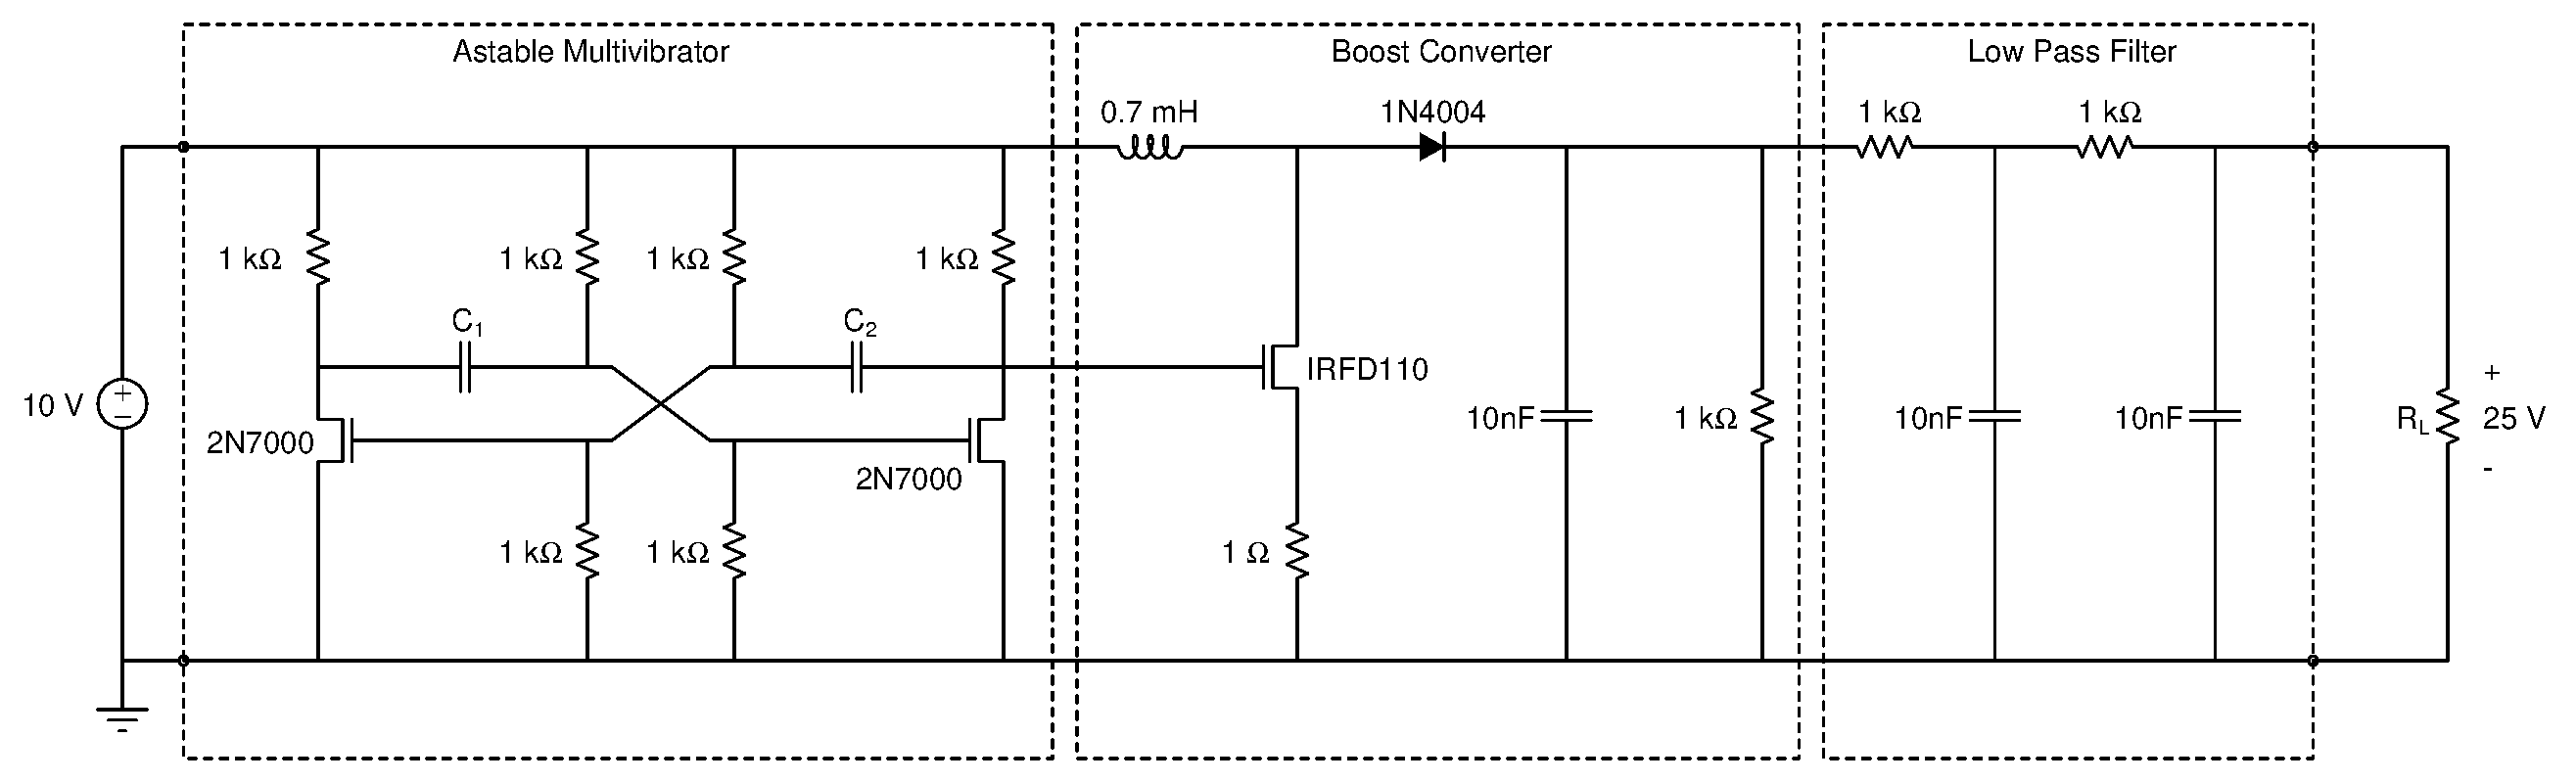
\includegraphics[width=6.5in]{dcdc}
\caption{Complete DC--DC power supply circuit schematic consisting of an astable multivibrator circuit, a boost converter circuit, and a low pass filter.}
\label{powersupply}
\end{figure}

When you’re describing how you made measurements, you do not need to be overly specific. For example, if you connected an oscilloscope to your circuit to measure voltage, you do not need to say, “One probe was connected to the resistor and the other probe was connected to ground.” Just say, “An oscilloscope was used to measure the voltage across the resistor.” The reader should have enough “know-how” to understand how you connect an oscilloscope to a circuit.

If you use an abbreviation such as MOSFET, make sure you define it before you use it. For example: A metal-oxide semiconducting field-effect transistor (MOSFET) is popular device for use in amplifiers and integrated circuits (ICs).

\subsection{Astable Multivibrator}

\subsection{Low Pass Filter}

\subsection{DC-DC Power Supply}

Make sure there are at least two subsections or subsubsections. If there is only one subsection, there is no need for that subsection.  
	
% Discussion
\section{Discussion}
\label{dis_section}

The end of the report is on the horizon! Use this blurb section to say things like, “Overall, the circuit operated as expected.” You can briefly touch on some good things and bad things.

Now is your chance to really discuss the lab. What happened? Did the circuit you built in lab operate as expected? Why? Why not? Integrate some circuit theory to explain deviations from expected results. If you messed up something, now is your chance to tell your TA you messed up. If you say how and why you messed up, you can still get some redemption points. So don’t skimp on this section! Also, it’s your chance to demonstrate that you really understood (well, hopefully you did) what went on in lab.

I like putting comparison tables in this section. Your TAs will like it too. Compare the calculated, simulated, and experimental results. Provide reasons for the deviations.

Summarize component values, results, and comparisons between theory, simulations, and measurements using tables.  In \LaTeX\, tables are easy to make and an example is illustrated below.  Always include units when presenting information in tables.

\begin{table}[ht]
\centering
\caption{Example table for the lab report.}
\begin{tabular}{ |c|c|c|c|c|p{2in}| } 
 \hline\hline
 Frequency (kHz) & Voltage (V) & Phase ($^\circ$) & Current (mA) & comment  \\\hline\hline 
 data1 & data2 & data3 & data4 & comment 1 \\ \hline
 data5 & data6 & data7 & data8 & comment 2\\ \hline
 data9  & daa10 & data11 & data12 & comment 3\\ 
 \hline\hline
\end{tabular}
\label{table_ex}
\end{table}

Take a look at the {\tt .tex} file to see how Table~\ref{table_ex} was created. Like figures, all tables should be referenced and described in the text.

You should always talk about sources of error and how they impacted the performance of the circuit. This section might get slightly repetitive with respect to your other discussion sections, but having a separate section devoted just to talking about sources of error is important. It also helps your TA see where you went wrong and where you know you went wrong. If you talk intelligently about your sources of error, you can get some redemption points if you messed up your lab. You should always have an idea of how to improve your circuit. Also, this is a chance to rack up some points.

\section{DC--DC Power Supply Cost Estimate}
\label{cost_section}

\section{Conclusions}
\label{con_section}

Yay! We’re done! Use the conclusion to tie up your report. Re-state the purpose of the lab and say whether or not you met the goals. Provide some of the major results and write a sentence or two about sources of error. In conclusion, I would like to apologize for doing all of the bad things I said not to do in your reports. These bad things include writing in first person and using conjunctions. This outline is more of “do as I say, not as I do” type of thing. Anyway, good luck with writing your own report.

% Appendices
 
\newpage
\begin{appendices}
\section{This is the first appendix}

Include any ancillary schematics, supporting data, and additional simulation results that help support your conclusions in appendices.

\section{This is the second appendix}
\end{appendices}

\newpage
% add a bibliography. Use the IEEE style guide for references.
\bibliographystyle{IEEEtran}  % IEEE Standard for bibliography
\bibliography{ECE214_Report} % Bibtex database file: "ECE214_Report.bib"


\end{document}
